\documentclass[a4paper,oneside]{scrartcl} %twocolumn,
\usepackage[utf8]{inputenc} %für MAC: applemac; für Windows: latin1 statt utf8
\usepackage[T1]{fontenc}
\usepackage[ngerman]{babel}

\usepackage{amsmath}
\usepackage{amsfonts}
\usepackage{amssymb}

\usepackage{mathptmx}
\usepackage{microtype}
\usepackage[nice]{nicefrac}

\usepackage{booktabs}

\usepackage{graphicx}

\usepackage{hyperref}

\setkomafont{captionlabel}{\upshape\bfseries}
\setkomafont{caption}{\itshape}


\title{Ultraschall}
\author{Robi Pedersen \and Simon Schmeißer}
\date{}

\begin{document}
\begin{titlepage}
  \maketitle
  \vfill
  \thispagestyle{empty}
  \begin{abstract}
    Hier sollte eine Zusammenfassung der Ergebnisse stehen. Der Umfang sollte dabei etwa 100 Wörte nicht überschreiten.
  \end{abstract}
\end{titlepage}

\tableofcontents
\clearpage
%*****************************************************************

\section{Aufgabenstellung}
\begin{enumerate}
 \item Bestimmung der Gitterkonstanten eines Sinusgitters aus dem Abstand der 1. Beugungsordnung.
\item Bestimmung der Gitterkonstanten von 5 Amplitudengittern.
\item Berechnung der Aperturfunktion für Gitter Nr.1 (größte Gitterkonstante,
      höchste Dichte an Beugungsmaxima) aus den ermittelten Intensitäten der
      Beugungsordnungen und Zeichnen einer Periode der Aperturfunktion.
\item Bestimmung des Verhältnisses der Spaltbreite zum Spaltabstand aus der
      Aperturfunktion.
\item Bestimmung des Auflösungsvermögens der Gitter bei ihrer vollen Ausleuchtung.

  \begin{enumerate}
    \item Messung der Intensitätsverteilung der Beugungsfigur eines Ultraschallwellengitters (Phasengitter)
	in Abhängigkeit von der Spannung am Ultraschallschwingquarz.
    \item Vergleich der Messergebnisse mit der Raman-Nath-Theorie.
    \item Bestimmung der Schallwellenlänge in Isooktan durch Ausmessen der Beugungsordnungen und Vergleich mit dem rechnerischen Wert.
  \end{enumerate}
\end{enumerate}

\section{Theorie}

\section{Versuchsbeschreibung}

\subsection{Versuchsaufbau}
\begin{figure}[h]
\centering 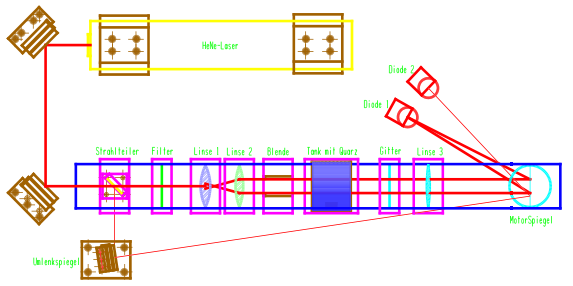
\includegraphics[width = \textwidth]{Bilder/Aufbau.jpg}
\caption{Schematischer Versuchsaufbau}
\end{figure}



\subsection{Durchf\"uhrung}

Mit einem He-Ne Laser, der monochromatisches Licht der Wellenl\"nge $\lambda = 6328 \mathring{A}$ abstrahlt, untersuchen wir das Beugungsph\"anomen an verschiedenen Gittern und bestimmen daraus die Gitterkonstanten bzw. Aperturfunktionen dieser Gitter. Bei einem Ultraschallgitter versuchen wir au\ss erdem die Schallwellenl\"ange in einer Isooktan-L\"osung herauszufinden und vergleichen unsere Messergebnisse mit der Raman-Nath-Theorie.

\subsubsection{Sinusgitter}

Wir richten den Laserstrahl senkrecht auf das Sinusgitter ohne Aufweitung und ohne Kollimationslinse, da bei diesem Gitter die 0. und die 1. Ordnung problemlos unterscheidbar sind. Auf einem Schirm hinter dem Gitter kann man das Beugungsmuster direkt beobachten und somit die Gitterkonstante bestimmen.

\subsubsection{Amplitudengitter}

Die H\"ohen der Linsen werden korrekt justiert und der Strahl wird durch Autokollimation auf Parallelit\"at \"uberpr\"uft. Dann wird der Drehspiegel eingesetzt und die Dioden werden so eingestellt, dass sie die maximale Signalintensit\"at aufnehmen k\"onnen. Schlussendlich eichen wir die Zeitachse des Oszilloskopenbildes anhand des Gitters "R". Anhand der Distanzen (Zeiten) zwischen dem Hauptmaximum und aller sichtbaren Beugungsordnungen auf dem Oszilloskop f\"ur alle Gitter, bestimmen wir durch lineare Regression die Umrechnungformel von Zeiten in Brechungswinkel.

\subsubsection{Aperturfunktion}

\clearpage

\section{Messwerte}

\section{Auswertung}

\section{Zusammenfassung}



\clearpage
%*****************************************************************
\appendix
Hier könntet ihr noch Bilder und Tabellen anhängen.
\clearpage


%*****************************************************************
\nocite{Raman}

\bibliographystyle{alpha}
\bibliography{bib}


\end{document}
